\documentclass{beamer}

\usepackage{txfonts}
\usepackage{hyperref}
\usepackage{fancybox}
\usepackage{xfrac}
\usepackage{cancel}

\newcommand{\heart}{\ensuremath\heartsuit}

\usepackage{mathtools,amssymb}
\newcommand{\myarrow}{\scalebox{2}[2]{$\mathclap{\curvearrowleft}\mkern2.2mu
                                                 \mathclap{\curvearrowright}$}}

\DeclareMathOperator{\Bin}{\mathrm{Bin}}

\hypersetup{colorlinks=false,linkbordercolor=red,linkcolor=green,pdfborderstyle={/S/U/W 1}}

\addtobeamertemplate{navigation symbols}{}{ \hspace{1em}    \usebeamerfont{footline}%
    \insertframenumber / \inserttotalframenumber}

\geometry{papersize={15cm,15cm}}
\usepackage{lipsum}

\makeatletter
\newenvironment<>{contdproof}[1][\proofname]{%
    \par
    \def\insertproofname{#1\@addpunct{.}}%
    \usebeamertemplate{proof begin}#2}
  {\usebeamertemplate{proof end}}
\makeatother


\setbeamertemplate{theorems}[numbered]

\newtheorem*{nonumdefinition}{Definition}
\newtheorem*{nonumproblem}{Problem}
\newtheorem*{nonumtheorem}{Theorem}
\newtheorem*{nonumremark}{Remark}
\newtheorem*{answer}{Answer}
\newtheorem*{nonumremarks}{Remarks}
\newtheorem*{nonumexamples}{Examples}
\newtheorem*{nonumsolution}{Solution}
\newtheorem*{nonumexample}{Example}
\newtheorem*{nonumproposition}{Proposition}
\newtheorem{proposition}[theorem]{Proposition}


\usepackage{tikz}
\newcommand*\mycirc[1]{%
  \tikz[baseline=(C.base)]\node[draw,circle,inner sep=.7pt](C) {#1};\:
}

\newcommand\myheading[1]{%
  \par\bigskip
  {\color{blue}{\large #1}}\par\smallskip}

%\usetheme{Warsaw}
%\usetheme{Berkeley} %sample 1

\usetheme{Berlin} % sample 2
%\usetheme{AnnArbor} % sample 3

\let\otp\titlepage
\renewcommand{\titlepage}{\otp\addtocounter{framenumber}{-1}}

\title{Lecture 8 : The Geometric Distribution}
\author{}
\date{}

\begin{document}
\begin{frame}[plain]
\titlepage
\end{frame}

\begin{frame}
The geometric distribution is a special case of negative binomial, it is the case $r=1$. It is so important we give it special treatment.

\myheading{Motivating example}

Suppose a couple decides to have children until they have a girl. Suppose the probability of having a girl is $P$. Let
$$
X=\text{the number of boys that precede the first girl}
$$
\end{frame}

\begin{frame}
Find the probability distribution of $X$. First $X$ could have any possible whole number value (although $X=1,000,000$ is very unlikely)

\medskip

\centerline{
\includegraphics[scale=1.1]{figure/fig1.eps}}
\smallskip

We have suppose birth are independent.

We have motivated.
\end{frame}

\begin{frame}
\begin{nonumdefinition}
Suppose a discrete random variable $X$ has the following $pmf$
$$
P(X=k)=q^{k}P, \ \ 0\leq k<\infty
$$
The $X$ is said to have geometric distribution with parameter $P$.
\end{nonumdefinition}

\begin{nonumremark}
Usually this is developed by replacing ``having a child'' by a Bernoulli experiment and having a girl by a ``success'' (PC). I could have used coin flips.
\end{nonumremark}
\end{frame}

\begin{frame}
\begin{nonumproposition}
Suppose $X$ has geometric distribution with parameter $p$.

Then
\begin{itemize}
\item[(i)] $E(X)=\dfrac{q}{p}$

\item[(ii)] $V(X)=\dfrac{q}{p^{2}}$
\end{itemize}
\end{nonumproposition}

\begin{proof}[Proof of (i) (you are not responsible for this)]
\begin{align*}
E(X) &= (0)(p)+(1)(qp)+(2)(q^{2}p)+\cdots+(k)(q^{k}p)+\cdots\\
     &= p(q+2q+\cdots+kq^{k}+\cdots
\end{align*}
Now 

\medskip
\centerline{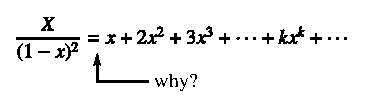
\includegraphics{figure/fig2.eps}}
\smallskip

So
$$
EX()=p\left(\dfrac{q}{(1-q)^{2}}\right)=p\left(\dfrac{q}{p^{2}}\right)=\dfrac{q}{p}
$$
\end{proof}
\end{frame}

\begin{frame}
\myheading{The Negative Binomial Distribution}

Now suppose the couple decides they want more girls - say $r$ girls, so they keep having children until the $r$-th girl appears. Let $X$ = the number of boys that precede the $r$-th girl.

Find the probability distribution of $X$.

\begin{nonumremark}
Sometimes (eg. pg. 13-14) it is better to write $X_{r}$ instead of $X$.
\end{nonumremark}
\end{frame}

\begin{frame}
Let's compute $P(X=k)$

\medskip
\centerline{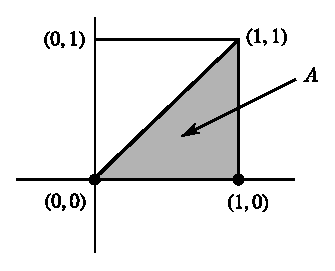
\includegraphics{figure/fig3.eps}}
\smallskip

What do we have preceding the $r$-th girl. Of course we must have $r-1$ girls and since we are assuming $X=k$ we have $k$ boys so $ktr-1$ children.

All orderings of boys and girls have the some probability so 
$$
P(X=k)=(?)P(\underbrace{B\ldots B}_{k-1} \underbrace{G\ldots G}_{r-1}G)
$$
\end{frame}

\begin{frame}
or
$$
P(X=k)=(?)q^{k}\cdot p^{r-1}\cdot q=(?)q^{k}p^{r}
$$
(?) is the number of words of length $ktr-1$ in $B$ and $G$ using $k$ $B$'s (where $r-1$ $G$'s).

Such a word is determined by choosing the slots occupied by the boys so there are $\binom{k+r-1}{k}$ words so
$$
P(X=k)=\binom{k+r-1}{k}p^{r}q^{k}
$$
\end{frame}

\begin{frame}
So we have motivated the following.

\begin{nonumdefinition}
A discrete random variable $X$ is said to have \underline{negative binomial distribution with parameters $r$ and $p$} if
$$
P(X=k)=\binom{k+r-1}{k} p^{r}q^{k}, \ 0\leq k<\infty
$$
The text denotes this proof by $nb(x;r,p)$ so 
$$
nb(x;r,p)=\binom{x+r-1}{k}p^{r}q^{x}, \ 0\leq x\leq \infty.
$$
\end{nonumdefinition}
\end{frame}

\begin{frame}
\begin{nonumproposition}
Suppose $X$ has negative binomial distribution with parameters $r$ and $p$. Then
\begin{itemize}
\item[(i)] $E(X)=r\dfrac{q}{p}$

\item[(ii)] $V(X)=\dfrac{rq}{p^{2}}$
\end{itemize}
\end{nonumproposition}
\end{frame}

\begin{frame}
\myheading{Waiting Times}

The binomial, geometric and negative binomial distributions are all tied to repeating a given Bernoulli experiment (flipping a coin, having a child) infinitely many times.

Think of discrete time $0,1,2,3,\ldots$ and we repeat the experiment at each of these discrete times. - Eg., flip a coin every minute.
\end{frame}

\begin{frame}
Now you can do the following things
\begin{enumerate}
\item Fix a time say $n$ and let $X=\sharp$ of successes in that time period. Then $X\sim \Bin (n,p)$. We should write $X_{n}$ and think of the family of random variable parametrized by the discrete time $n$ as the ``binomial process''. (see page. 18 - the Poisson process).

\item ((discrete) waiting time for the first success) 

Let $Y$ be the amount of time up to the time the first success occurs.
\end{enumerate}
\end{frame}

\begin{frame}
This is the geometric random variable. Why?

Suppose we have in out boy/girl example
$$
\underbrace{\frac{B}{0} \ \frac{B}{1} \ \frac{B}{2} \ \frac{}{3} \ \frac{B}{}}_{k} \ \frac{G}{k}
$$
So in this case 

$X=\sharp$ of boys = $k$

$Y$ = waiting time = $k$

so $Y=X$.
\end{frame}

\begin{frame}
\myheading{Waiting time for $r$-th success}

Now let $Y_{n}=$ the waiting time up to the $r$-th success then there is a difference between $X_{r}$ and $Y_{r}$.

Suppose $X_{r}=k$ so there are $k$ boys before the $r$-th girl arrives.
$$
\underbrace{\frac{}{0} \ \frac{B}{1} \ \frac{}{2} \ \frac{}{} \ \frac{}{} \ \frac{}{} \ \frac{}{k+r-2}} \ \frac{G}{k+r-1}
$$
$k$ $B$'s $r-1$ $G$'s so $ktr-1$ slots.

But start at $0$ so the last slot is $k+r-\mycirc{2}$ so
$$
Y_{r}=X_{r}+r-1
$$
\end{frame}

\begin{frame}
\myheading{The Poisson Distribution}

For a change we won't start with a motivating example but will start with the definition.

\begin{nonumdefinition}
A discrete random variable $X$ is said to have Poisson distribution with parameter $\lambda$.
$$
P(X=k)=e^{-\lambda}\dfrac{\lambda^{k}}{k!}, \ 0\leq k<\infty
$$
We will abbreviate this to $X\sim P(\lambda)$.

I will now try to motivate the formula which looks complicated.
\end{nonumdefinition}
\end{frame}

\begin{frame}
Why is the factor of $e^{-\lambda}$ there? It is there to make to total probability equal to $1$.

Total Probability $=\sum\limits^{\infty}_{k=0}P(X=k)$
$$
=\sum\limits^{\infty}_{k=0}e^{-\lambda}\dfrac{\lambda^{k}}{k!}=e^{-\lambda}\sum\limits^{\infty}_{k=0}\dfrac{\lambda^{k}}{k!}
$$
But from calculus
$$
e^{X}=\sum\limits^{\infty}_{k=0}\dfrac{X^{k}}{k!}
$$
Total probability $=e^{-\alpha}\cdot e^{\alpha}=1$ as it has to be.
\end{frame}

\begin{frame}
\begin{nonumproposition}
Suppose $X\sim P(\lambda)$. Then
\begin{itemize}
\item[(i)] $E(X)=\lambda$

\item[(ii)] $V(X)=\lambda$
\end{itemize}
\end{nonumproposition}

\begin{nonumremark}
It is remarkable that $E(X)=V(X)$.
\end{nonumremark}

\begin{nonumexample}[3.39]
Let $X$ denote the number of creatures of a particular type captured during a given time period. Suppose $X\sim P(4.5)$. Find $P(X=5)$ and $P(X\leq 5)$.
\end{nonumexample}
\end{frame}

\begin{frame}
\begin{nonumsolution}
$$
P(X=5)=e^{-4.5}\frac{(4.5)^{5}}{5!}
$$
(just plug into the formula using $\lambda=4.5$)
\begin{align*}
P(X\leq 5) &= P(X=0)+P(X=1)+P(X=2)\\
           &\quad +P(X=3)+P(X-4)+P(X=5)\\
           &= e^{-\lambda}+e^{-\lambda}\lambda +e^{-\lambda}\frac{\lambda^{2}}{2}\\
           &\quad \underbrace{+e^{-\lambda}\frac{\lambda^{3}}{3!}+e^{-\lambda}\frac{\lambda^{4}}{4!}+e^{-\lambda^{2}}\frac{\lambda^{5}}{5!}}_{\text{don't try to evaluate this}}
\end{align*}
\end{nonumsolution}
\end{frame}

\begin{frame}
\myheading{The Poisson Process}

A very important application of the Poisson distribution arises in counting the number of occurrences of a certain event in time $t$
\begin{enumerate}
\item Animals in a trap.

\item Calls coming into a telephone switch board.
\end{enumerate}
Now we could let $t$ vary so we get a one-parameter family of Poisson random variable $X_{t}$, $0\leq t<\infty$.

Now a Poisson process is completely determined once we know its mean $\lambda$.
\end{frame}

\begin{frame}
So far each $t$, $X_{t}$ is a Poisson random variable. So $X_{t}\sim P(\lambda(t))$.

So the Poisson parameter $\lambda$ is a function of $t$.

In the \underline{Poisson process} one assume that $\lambda(t)$ is the simplest possible function of $t$ (aside from a constant function) namely a linear function
$$
\lambda(t)=\alpha t.
$$
Necessarily 
$$
\alpha=\lambda(1)=\text{the average number of observations in unit time.}
$$
\end{frame}

\begin{frame}
\begin{nonumremark}
In the text, page 124, the author proposes 3 axioms on a one parameter family of random variables $X_{t}$. So that $X_{t}$ is a Poisson process i.e.,
$$
X_{t}\sim P(\alpha t)
$$
\end{nonumremark}

\begin{nonumexample}
(from an earlier version of the text)

The number of tickets issued by a meter reader can be modelled by a Poisson process with a rate of 10 ticket every two pairs.
\end{nonumexample}
\end{frame}

\begin{frame}
(a) What is the probability that exactly 10 tickets are given out during a particular 12 hour period.

\begin{nonumsolution}
We want $P(X_{12}=10)$. 

First find $\alpha$ = average $\sharp$ of tickets by unit time.

So \ $\alpha=\dfrac{10}{2}=5$

So \ $X_{t}\sim P(5t)$
\end{nonumsolution}
\end{frame}

\begin{frame}
\begin{nonumsolution}[Cont.]
So \ $X_{12}\sim P((5)(12))=P(60)$
\begin{align*}
P(X_{12}=10) &= e^{-\lambda}\frac{\lambda^{10}}{(10)!}\\[3pt]
            &= e^{-60}\frac{(60)^{10}}{(10)!}
\end{align*}
\end{nonumsolution}

(b) What is the probability that at least 10 tickets are given out during a 12 hour time period.
\end{frame}

\begin{frame}
We wait
\begin{align*}
& P(X_{12}\geq 10)=1-P(X\leq 9)\\[3pt]
&\quad =1-\sum\limits^{9}_{k=0}e^{-\lambda}\frac{\lambda^{k}}{k!}\\[3pt]
&\quad =1-\underbrace{\sum\limits^{9}_{k=0}e^{-60}\frac{(60)^{k}}{k!}}_{\substack{\text{not something you}\\ \text{want to try to}\\ \text{evaluate by hand.}}}
\end{align*}
\end{frame}

\begin{frame}
\myheading{Waiting Times}

Again there are waiting time random variables associated to the Poisson process.

Let $Y$ = waiting time until the first animal is caught in the trap.

and $Y_{r}$ = waiting time until the $r$-th animal is caught in the trap.

Now $Y$ and $Y_{r}$ are \underline{continuous} random variables which we are about to study. $Y$ is \underline{exponential} and $Y_{r}$ has a special kind \underline{gomma} distribution.
\end{frame}
\end{document}


